\documentclass[usenames,dvipsnames,aspectratio=169]{beamer}
\usepackage{../common/prgBasics}

\usepackage{array}
\newcolumntype{C}[1]{>{\centering\let\newline\\\arraybackslash\hspace{0pt}}m{#1}}

\title[Lecture 10.]{Programming basics}
\subtitle{(GKNB\_INTA023)}

\begin{document}

%1
\begin{frame}[plain]
  \titlepage
\end{frame}

%2
\begin{frame}{Macros with arguments}
  Problem:
  \begin{itemize}
    \item[] If a function is very simple, the \emph{time of invocation} is comparable with the \emph{time of operation} $\to$ ineffectice, slow programs
  \end{itemize}
  Solution:
  \begin{itemize}
    \item[] Change function calls to macro substitution! $\to$ text replacement with the preprocessor
  \end{itemize}
\end{frame}

%3
\begin{frame}{Macros with arguments}
  \footnotesize
  \begin{exampleblock}{\textattachfile{operation1.c}{operation1.c}}
    \lstinputlisting[style=c]{operation1.c}
  \end{exampleblock}
  \vfill
  \normalsize
  Task: substitute all function calls with macros!\\
  \scriptsize 
  \texttt{\#define \emph{name}(\emph{identifier-list}) \emph{preprocessor-symbols}} \emph{newline}
\end{frame}

%4
\begin{frame}{Macros with arguments}
  \kiemel{Caution!} \\
  \small
  It is forbidden to put a whitespace character between \kiemel{\texttt{SQUARE}} and \kiemel{\texttt{(}}! $\to$ changes the meaning to simple macro substitution, without arguments
  \scriptsize
  \begin{exampleblock}{\textattachfile{operation2.c}{operation2.c}}
    \lstinputlisting[style=c]{operation2.c}
  \end{exampleblock}
  \vfill
  \normalsize
  Problem: order of operations!\\
  Solution: brackets
\end{frame}

%5
\begin{frame}{Macros with arguments}
  \scriptsize
  \begin{exampleblock}{\textattachfile{operation3.c}{operation3.c}}
    \lstinputlisting[style=c]{operation3.c}
  \end{exampleblock}
  \vfill
  \normalsize
  Next task: write a macro for addition!
\end{frame}

%6
\begin{frame}{Macros with arguments}
  \scriptsize
  \begin{exampleblock}{\textattachfile{operation4.c}{operation4.c}}
    \vspace{-.3cm}
    \lstinputlisting[style=c,linerange={3-18},firstnumber=3]{operation4.c}
    \vspace{-.3cm}
  \end{exampleblock}
  \vfill
  Problem: actual parameters are evaluated before function invocation, but are used without any modifications in case of macros $\to$ different program behavior, misleading\\
  Solution: further brackets
\end{frame}

%7
\begin{frame}{Macros with arguments}
  \scriptsize
  \begin{exampleblock}{\textattachfile{operation5.c}{operation5.c}}
    \lstinputlisting[style=c,linerange={3-18},firstnumber=3]{operation5.c}
  \end{exampleblock}
\end{frame}

%8
\begin{frame}{Macros with arguments}
  Task: modify our earlier matrix addition program to calculate indexes with a macro!
  \scriptsize
  \begin{exampleblock}{\textattachfile{mtxAdd5.c}{mtxAdd5.c}}
    \lstinputlisting[style=c,linerange={5-19},firstnumber=5]{mtxAdd5.c}
  \end{exampleblock}
\end{frame}

%9
\begin{frame}{Macros with arguments}
  Pros:
  \begin{itemize}
    \item Faster than a function call
    \item The code is less type-dependent
  \end{itemize}
  \vfill
  Cons:
  \begin{itemize}
    \item No type checks, hard to explore mistakes
    \item Code size increases, it is not suitable to replace complex functions
    \item The evaluation of passed expressions happens several times $\to$ time, side effects
  \end{itemize}
\end{frame}

%10
\begin{frame}{Sorting names}
  Task:
  \begin{itemize}
    \item Read names and list them in alphabetical order!
    \item For the sake of simplicity, store the characters of names in a two-dimensional array
  \end{itemize}
  \begin{center}
    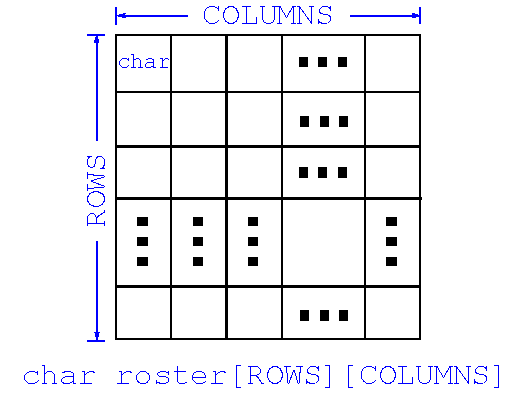
\includegraphics[scale=0.75]{roster1.pdf}
  \end{center}
\end{frame}

%11
\begin{frame}{Sorting names}
  \begin{exampleblock}{\textattachfile{roster1.c}{roster1.c}}
    \lstinputlisting[style=c,linerange={4-5},firstnumber=4]{roster1.c}
    \lstinputlisting[style=c,linerange={47-55},firstnumber=47]{roster1.c}
  \end{exampleblock}
\end{frame}

%12
\begin{frame}{Sorting names}
  \begin{exampleblock}{\textattachfile{roster1.c}{roster1.c}}
    \lstinputlisting[style=c,linerange={16-26},firstnumber=16]{roster1.c}
  \end{exampleblock}
\end{frame}

%13
\begin{frame}{Sorting names}
  \begin{exampleblock}{\textattachfile{roster1.c}{roster1.c}}
    \lstinputlisting[style=c,linerange={28-39},firstnumber=28]{roster1.c}
  \end{exampleblock}
\end{frame}

%14
\begin{frame}{Sorting names}
  \begin{exampleblock}{\textattachfile{roster1.c}{roster1.c}}
    \lstinputlisting[style=c,linerange={41-45},firstnumber=41]{roster1.c}
  \end{exampleblock}
\end{frame}

%15
\begin{frame}{Sorting names}
  Problem:
  \begin{itemize}
    \item[] The length of lines is the same $\to$ sometimes more memory would be needed, sometimes it is already too much
  \end{itemize}
  Task:
  \begin{itemize}
    \item[] Modify the data structure, use an array of char pointers and allocate memory for the lines runtime!
  \end{itemize}
  \begin{center}
    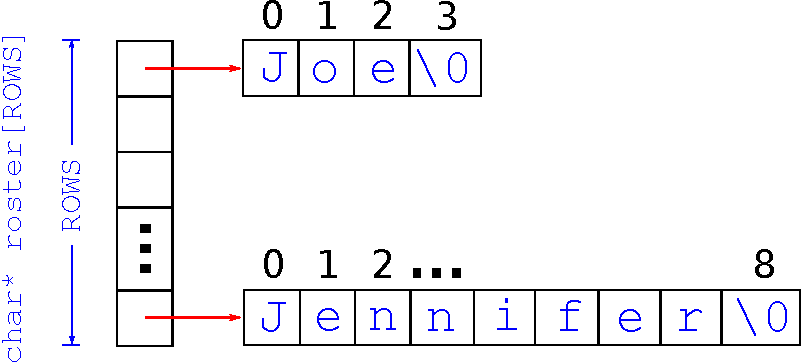
\includegraphics[scale=0.6]{roster2.pdf}
  \end{center}
\end{frame}

%16
\begin{frame}{Sorting names}
  \begin{exampleblock}{\textattachfile{roster2.c}{roster2.c}}
    \lstinputlisting[style=c,linerange={5-5},firstnumber=5]{roster2.c}
    \lstinputlisting[style=c,linerange={56-65},firstnumber=56]{roster2.c}
  \end{exampleblock}
\end{frame}

%17
\begin{frame}{Sorting names}
  \footnotesize
  \begin{exampleblock}{\textattachfile{roster2.c}{roster2.c}}
    \lstinputlisting[style=c,linerange={16-30},firstnumber=16]{roster2.c}
  \end{exampleblock}
\end{frame}

%18
\begin{frame}{Sorting names}
  \footnotesize
  \begin{exampleblock}{\textattachfile{roster2.c}{roster2.c}}
    \vspace{-.3cm}
    \lstinputlisting[style=c,linerange={32-42},firstnumber=32]{roster2.c}
    \lstinputlisting[style=c,linerange={50-54},firstnumber=50]{roster2.c}
    \vspace{-.3cm}
  \end{exampleblock}
\end{frame}

%19
\begin{frame}{Sorting names}
  Problem:
  \begin{itemize}
    \item[] The number of names is still limited
  \end{itemize}
  Task:
  \begin{itemize}
    \item[] Allocate memory for the pointer array at runtime!
  \end{itemize}
  \footnotesize
  \begin{exampleblock}{\textattachfile{roster3.c}{roster3.c}}
    \lstinputlisting[style=c,linerange={56-65},firstnumber=56]{roster3.c}
  \end{exampleblock}
\end{frame}

%20
\begin{frame}{Sorting names}
  \footnotesize
  \begin{exampleblock}{\textattachfile{roster3.c}{roster3.c}}
    \lstinputlisting[style=c,linerange={15-29},firstnumber=15]{roster3.c}
  \end{exampleblock}
\end{frame}

%21
\begin{frame}{Sorting names}
  \footnotesize
  \begin{exampleblock}{\textattachfile{roster3.c}{roster3.c}}
    \lstinputlisting[style=c,linerange={43-54},firstnumber=43]{roster3.c}
  \end{exampleblock}
\end{frame}

%22
\begin{frame}{Distances of cities}
  Task:
  \begin{itemize}
    \item Reading the names of two cities
    \item Printing the distance of these cities
    \item Exit if the same city is entered twice
  \end{itemize}
  \vfill
  Solution:
  \begin{itemize}
    \item Storing the names of cities in a vector
    \item and the distances of cities in a matrix
    \item The same index can be used to access the name of the city and it's distance from another city
  \end{itemize}
\end{frame}

%23
\begin{frame}[fragile]{Distances of cities}
  \begin{block}{Output}
    \begin{verbatim}
Determining the distances of cities
Exit by entering the same city twice
Departure from: Budapest
Arrival at: Eldorado
Non-existent city!
Gyor
Distance: 121km
Departure from: Gyor
Arrival at: Gyor
\end{verbatim}
  \end{block}
\end{frame}

%24
\begin{frame}{Distances of cities}
  \begin{exampleblock}{\textattachfile{cities1.c}{cities1.c}}
    \footnotesize
    \lstinputlisting[style=c,linerange={48-60},firstnumber=48]{cities1.c}
  \end{exampleblock}
\end{frame}

%25
\begin{frame}{Distances of cities}
  \begin{exampleblock}{\textattachfile{cities1.c}{cities1.c}}
    \scriptsize
    \vspace{-.3cm}
    \lstinputlisting[style=c,linerange={15-33},firstnumber=15]{cities1.c}
    \vspace{-.3cm}
  \end{exampleblock}
\end{frame}

%26
\begin{frame}{Distances of cities}
  \begin{exampleblock}{\textattachfile{cities1.c}{cities1.c}}
    \vspace{-.3cm}
    \lstinputlisting[style=c,linerange={35-46},firstnumber=35]{cities1.c}
    \vspace{-.3cm}
  \end{exampleblock}
\end{frame}

%27
\begin{frame}{``Triangular'' matrices}
  Remark: more than the half of the data in the matrix can be omitted\\
  \qquad ($m_{i,j}=m_{j,i}, m_{i,i} = 0$)
  \begin{center}
    \small
    \begin{tabular}{r|ccccccc}
                  & \rotatebox{90}{Budapest} & \rotatebox{90}{Győr} & \rotatebox{90}{Szeged} &
                    \rotatebox{90}{Debrecen} & \rotatebox{90}{Veszprém} & \rotatebox{90}{Dunaújváros} &
                    \rotatebox{90}{Eger} \\ \hline
      Budapest    & \kiemelZ{0}  & 121 & 174 & 231 & 115 &  83 & 139 \\
      Győr        & \kiemel{121} & \kiemelZ{0}  & 287 & 377 &  82 & 176 & 285 \\
      Szeged      & \kiemel{174} & \kiemel{287} & \kiemelZ{0}  & 218 & 278 & 161 & 298 \\
      Debrecen    & \kiemel{231} & \kiemel{377} & \kiemel{218} & \kiemelZ{0}  & 368 & 320 & 131 \\
      Veszprém    & \kiemel{115} & \kiemel{82}  & \kiemel{278} & \kiemel{368} & \kiemelZ{0}  & 103 & 275 \\
      Dunaújváros & \kiemel{83}  & \kiemel{176} & \kiemel{161} & \kiemel{320} & \kiemel{103} & \kiemelZ{0}  & 228 \\
      Eger        & \kiemel{139} & \kiemel{285} & \kiemel{298} & \kiemel{131} & \kiemel{275} & \kiemel{228} & \kiemelZ{0} \\
    \end{tabular}
  \end{center}
  Problem: all rows of a matrix have the same length\\
  Solution: creating a vector addressing vectors of different lengths\\
  \qquad \small (array of pointers, $\approx$ lower triangular matrix)
\end{frame}

%28
\begin{frame}{``Triangular'' matrices}
  \begin{exampleblock}{\textattachfile{cities2.c}{cities2.c}}
    \footnotesize
    \vspace{-.3cm}
    \lstinputlisting[style=c,linerange={35-50},firstnumber=24]{cities2.c}
    \vspace{-.3cm}
  \end{exampleblock}
\end{frame}

%29
\begin{frame}{Alternative solution}
  Remark: even the pointers to vectors can be saved if the values under the main diagonal are stored continuously in a single vector
  \begin{center}
    \scriptsize
    \begin{tabular}{r|cccccc}
                  & \rotatebox{90}{Bp. [0]} & \rotatebox{90}{Győr [1]} & \rotatebox{90}{Szeged [2]} &
                    \rotatebox{90}{Debr. [3]} & \rotatebox{90}{Veszp. [4]} & \rotatebox{90}{Duv. [5]}\\ \hline
      Győr [1]        & \kiemelZ{121} & & & & & \\
      Szeged [2]      & \kiemelZ{174} & \kiemelZ{287} & & & & \\
      Debrecen [3]    & \kiemelZ{231} & \kiemelZ{377} & \kiemelZ{218} & & & \\
      Veszprém [4]    & \kiemel{115} & \kiemel{82} & 278 & 368 & & \\
      Dunaújváros [5] & 83 & 176 & 161 & 320 & 103 & \\
      Eger [6]        & 139 & 285 & 298 & 131 & 275 & 228 \\
    \end{tabular}\\
    \vspace{.3cm}
    \begin{tabular}{c|cc|ccc|cccc}
      [0] & [1] & [2] & [3] & [4] & [5] & [6] & [7] & [8] & [9] \\ \hline
      \kiemelZ{121} & \kiemelZ{174} & \kiemelZ{287} & \kiemelZ{231} & \kiemelZ{377} & \kiemelZ{218} & 
        \kiemel{115} & \kiemel{82} & 278 & \dots \\
    \end{tabular}
  \end{center}
  The number of distances in rows above the searched data forms an arithmetical progression
  $\to S_n = \frac{[2a_1 + (n-1)d] \cdot n}{2}$, specifically $a_1=1, d=1 \to S_n = \frac{(n+1) \cdot n}{2}$
\end{frame}

%30
\begin{frame}{Alternative solution}
  \tiny
  \kiemel{Watch out!} The indexing of rows in the program starts with 0, not with 1!
  \begin{exampleblock}{\textattachfile{cities3.c}{cities3.c}}
    \scriptsize
    \lstinputlisting[style=c,linerange={35-51},firstnumber=35]{cities3.c}
  \end{exampleblock}
\end{frame}

%31
\begin{frame}{Static variables}
  Problem:
  \begin{itemize}
    \item local variables have \emph{automatic} lifetime (\texttt{auto}): from the moment of definition to the moment when execution leaves their block
    \item re-allocation of vectors and matrices are time consuming
  \end{itemize}
  \vfill
  Solution: usage of the \texttt{static} modifier
  \begin{itemize}
    \item lifetime: from the start of the program to its end $\to$ keep their values between function calls
    \item scope: unchanged (from declaration to the end of the block)
    \item initialized implicitely (filling with zero bits)
  \end{itemize}
\end{frame}

%32
\begin{frame}{Static variables}
  \begin{exampleblock}{\textattachfile{cities4.c}{cities4.c}}
    \scriptsize
    \lstinputlisting[style=c,linerange={35-51},firstnumber=35]{cities4.c}
  \end{exampleblock}
\end{frame}

%33
\begin{frame}{Dynamic ``Triangle matrices''}
  Task: 
  \begin{itemize}
    \item Create the vector and the triangle matrix at runtime
    \item Fill them with values given by the user
  \end{itemize}
  \begin{exampleblock}{\textattachfile{cities5.c}{cities5.c} -- \texttt{main}}
    \scriptsize
    \lstinputlisting[style=c,linerange={74-85},firstnumber=74]{cities5.c}
  \end{exampleblock}
\end{frame}

%34
\begin{frame}{Dynamic ``Triangle matrices''}
  \begin{exampleblock}{\textattachfile{cities5.c}{cities5.c} -- \texttt{main}}
    \footnotesize
    \lstinputlisting[style=c,linerange={86-98},firstnumber=86]{cities5.c}
  \end{exampleblock}
\end{frame}

%35
\begin{frame}{Dynamic ``Triangle matrices''}
  \small
  \begin{exampleblock}{\textattachfile{cities5.c}{cities5.c}}
    \lstinputlisting[style=c,linerange={16-27},firstnumber=16]{cities5.c}
  \end{exampleblock}
\end{frame}

%36
\begin{frame}{Dynamic ``Triangle matrices''}
  \begin{exampleblock}{\textattachfile{cities5.c}{cities5.c}}
    \lstinputlisting[style=c,linerange={41-52},firstnumber=41]{cities5.c}
  \end{exampleblock}
\end{frame}

%37
\begin{frame}{Dynamic ``Triangle matrices''}
  \footnotesize
  \begin{exampleblock}{\textattachfile{cities5.c}{cities5.c}}
    \lstinputlisting[style=c,linerange={29-39},firstnumber=29]{cities5.c}
  \end{exampleblock}
\end{frame}

%38
\begin{frame}{Dynamic ``Triangle matrices''}
  \begin{exampleblock}{\textattachfile{cities5.c}{cities5.c}}
    \lstinputlisting[style=c,linerange={54-62},firstnumber=54]{cities5.c}
  \end{exampleblock}
\end{frame}

%39
\begin{frame}{Dynamic ``Triangle matrices''}
  \begin{exampleblock}{\textattachfile{cities5.c}{cities5.c}}
    \lstinputlisting[style=c,linerange={64-72},firstnumber=64]{cities5.c}
  \end{exampleblock}
\end{frame}

%40
\begin{frame}{Magic square}
  \begin{itemize}
    \item A square matrix containing (generally between 1 and $n^2$) integers in which
    \begin{itemize}
      \item the sum of all rows,
      \item the sum of all columns,
      \item the sum of numbers on the main diagonal and
      \item the sum of numbers on the side diagonal are the same.
    \end{itemize}
    \item \hiv{\href{http://en.wikipedia.org/wiki/Magic_square}{Further curiosities}}
  \end{itemize}
  \begin{center}
    \tiny
    \begin{tabular}{cc}
      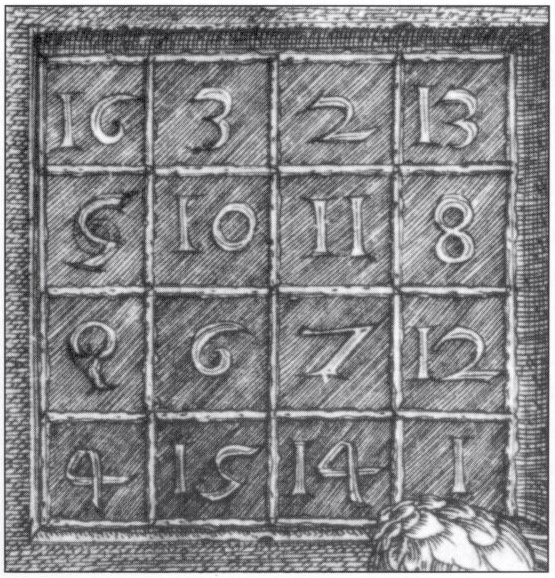
\includegraphics[height=3cm]{melancolia.jpg} & 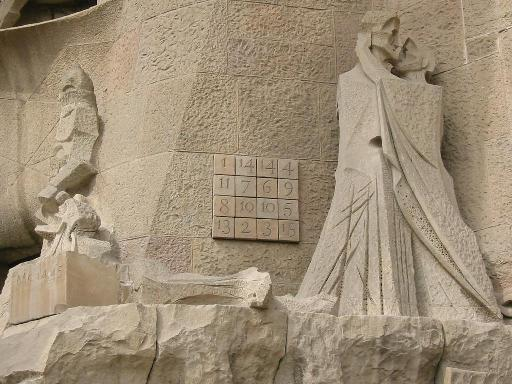
\includegraphics[height=3cm]{sagrada.jpg} \\
      Albrecht Dürer: Melencolia I (detail) & Sagrada Família, Barcelona\\
    \end{tabular}
  \end{center}
\end{frame}

%41
\begin{frame}{Magic square}
  \scriptsize
 \hiv{\href
 {https://en.wikipedia.org/wiki/Magic_square\#A_method_for_constructing_a_magic_square_of_odd_order}
 {Constructing a magic square of odd order}}
  \begin{enumerate}
    \item Start in the central column of the first row with the number 1
    \item Write increasing numbers in the matrix during the consecutive steps (2, 3, \dots,
$n^2$)!
    \item The place of the next value is in general \kiemel{one step upwards and to the right}
    \begin{itemize}
      \scriptsize
      \item If the determined element is already filled the operation must be continued \kiemel{below} the previously filled element
      \item If the determined element lies outside the matrix move to the \kiemel{opposite side} (eg. instead of the element ``above the topmost one'' use the element at the bottom).
    \end{itemize}
  \end{enumerate}
  \begin{center}
    \begin{tabular}{|C{.2cm}|C{.2cm}|C{.2cm}|}
      \hline
      \multicolumn{3}{|c|}{Step 1}\\
      \hline
       & 1 &  \\
      \hline
       &  &  \\
      \hline
       &  &  \\
      \hline
    \end{tabular}
    \begin{tabular}{|C{.2cm}|C{.2cm}|C{.2cm}|}
      \hline
      \multicolumn{3}{|c|}{Step 2}\\
      \hline
       & 1 &  \\
      \hline
       &  &  \\
      \hline
       &  & 2 \\
      \hline
    \end{tabular}
    \begin{tabular}{|C{.2cm}|C{.2cm}|C{.2cm}|}
      \hline
      \multicolumn{3}{|c|}{Step 3}\\
      \hline
       & 1 &  \\
      \hline
      3 &  &  \\
      \hline
       &  & 2 \\
      \hline
    \end{tabular}
    \begin{tabular}{|C{.2cm}|C{.2cm}|C{.2cm}|}
      \hline
      \multicolumn{3}{|c|}{Step 4}\\
      \hline
       & 1 &  \\
      \hline
      3 &  &  \\
      \hline
      4 &  & 2 \\
      \hline
    \end{tabular}
    \begin{tabular}{|C{.2cm}|C{.2cm}|C{.2cm}|}
      \hline
      \multicolumn{3}{|c|}{Step 5}\\
      \hline
       & 1 &  \\
      \hline
      3 & 5 &  \\
      \hline
      4 &  & 2 \\
      \hline
    \end{tabular}
    \begin{tabular}{|C{.2cm}|C{.2cm}|C{.2cm}|}
      \hline
      \multicolumn{3}{|c|}{Step 6}\\
      \hline
       & 1 & 6 \\
      \hline
      3 & 5 &  \\
      \hline
      4 &  & 2 \\
      \hline
    \end{tabular}
    \begin{tabular}{|C{.2cm}|C{.2cm}|C{.2cm}|}
      \hline
      \multicolumn{3}{|c|}{Step 7}\\
      \hline
       & 1 & 6 \\
      \hline
      3 & 5 & 7 \\
      \hline
      4 &  & 2 \\
      \hline
    \end{tabular}
    \begin{tabular}{|C{.2cm}|C{.2cm}|C{.2cm}|}
      \hline
      \multicolumn{3}{|c|}{Step 8}\\
      \hline
      8 & 1 & 6 \\
      \hline
      3 & 5 & 7 \\
      \hline
      4 &  & 2 \\
      \hline
    \end{tabular}
    \begin{tabular}{|C{.2cm}|C{.2cm}|C{.2cm}|}
      \hline
      \multicolumn{3}{|c|}{Step 9}\\
      \hline
      8 & 1 & 6 \\
      \hline
      3 & 5 & 7 \\
      \hline
      4 & 9 & 2 \\
      \hline
    \end{tabular}
  \end{center}
\end{frame}

%42
\begin{frame}{Magic square}
  \begin{exampleblock}{\textattachfile{magic.c}{magic.c}}
    \lstinputlisting[style=c,linerange={43-53},firstnumber=43]{magic.c}
  \end{exampleblock}
\end{frame}

%43
\begin{frame}{Magic square}
  \small
  \begin{exampleblock}{\textattachfile{magic.c}{magic.c} -- \texttt{generate}}
    \lstinputlisting[style=c,linerange={4-10},firstnumber=4]{magic.c}
  \end{exampleblock}
\end{frame}

%44
\begin{frame}{Magic square}
  \begin{exampleblock}{\textattachfile{magic.c}{magic.c} -- \texttt{generate}}
    \footnotesize
    \lstinputlisting[style=c,linerange={11-25},firstnumber=11]{magic.c}
  \end{exampleblock}
\end{frame}

%45
\begin{frame}{Magic square}
  \begin{exampleblock}{\textattachfile{magic.c}{magic.c}}
    \footnotesize
    \lstinputlisting[style=c,linerange={27-41},firstnumber=27]{magic.c}
  \end{exampleblock}
\end{frame}

\end{document}
